\documentclass[11pt]{article}

\usepackage[letterpaper]{geometry}

\usepackage[utf8]{inputenc}
\usepackage{mathpazo}
\usepackage{amsmath}
\usepackage{amsfonts}
\usepackage{physics}
\usepackage{siunitx}

\usepackage{fancyhdr}

\usepackage{graphicx}
\usepackage{float}
\usepackage{booktabs}

\usepackage[shortlabels,inline]{enumitem}

% Hyperlinks with decent looking default colors.
\usepackage{hyperref}
\usepackage{xcolor}
\hypersetup{
  colorlinks,
  linkcolor={red!50!black},
  citecolor={blue!50!black},
  urlcolor={blue!80!black}
}

% For those sexy spaced low small caps from classic-thesis!
\usepackage{microtype}
\usepackage{textcase}
\DeclareRobustCommand{\spacedlowsmallcaps}[1]{%
  \textls[80]{\scshape\MakeTextLowercase{#1}}%
}

% Replaced mathpazo \sum symbol with computer modern's.
\DeclareSymbolFont{cmlargesymbols}{OMX}{cmex}{m}{n}
\let\sumop\relax
\DeclareMathSymbol{\sumop}{\mathop}{cmlargesymbols}{"50}

\newcommand{\forceindent}{\leavevmode{\parindent=1em\indent}}

\pagestyle{fancy} 
\fancyhead{}
\rhead{Ali Ramadhan}
\chead{}
\lhead{12.818: Project 4}
\cfoot{}
\rfoot{\thepage}

\title{\spacedlowsmallcaps{\small 12.818: Introduction to Atmospheric Data and Large-scale Dynamics}\\ \spacedlowsmallcaps{\Large Project four: The meridional structure of the atmosphere}}
\author{\spacedlowsmallcaps{Ali Ramadhan}}
\date{}

% \renewcommand\thesection{\Alph{section}}

\begin{document}
\maketitle

In this project we will investigate the meridional structure and circulation of the atmosphere. To do so we have started by plotting the zonally averaged air temperature $T$ (figure \ref{fig:airT}), potential temperature $\theta$ (figure \ref{fig:theta}), specific humidity $q$ (figure \ref{fig:qstar}), meridional wind velocity (figure \ref{fig:mer_wind}), zonal wind velocity (figure \ref{fig:zonal_wind}), and vertical velocity $\omega$ in \SI{}{\Pa/s} (figure \ref{fig:omega})). Each variable is plotted for the month of January (top panel of each figure) and July (bottom panel of each figure). The figures were produced using NCEP reanalysis data averaged over the years 1948--2017 \cite{Kalnay}.

Looking at the zonally averaged temperatures in figure \ref{fig:airT}, we see that the tropospheric temperature are indeed higher in the tropics during both January and July. Stratospheric temperatures are higher at the poles, and in particular at the pole with the greater insolation, so the stratosphere is warmest over the South Pole in January when the Antarctic continent is continuously bathed in stellar radiation, and the stratosphere is warmest over the North Pole in July.

If the Earth were not rotating then this temperature difference would set up a circulation in which warm air rises at low latitudes and cold air sinks at high latitudes. This would essentially result in Hadley cells that extend much closer to the poles as the Coriolis effect would not be there to deflect the air masses. However, we see little evidence of this kind of cell as air mainly sinks in the mid-latitudes below \SI{30}{\degree N} (see figure \ref{fig:omega}). There is some sinking of air near the poles but it is also accompanied by adjacent rising from further south, forming a completely different cell called the polar cell.

Comparing the zonally averaged temperature (figure \ref{fig:airT}) and potential temperature (figure \ref{fig:theta}) we immediately see that while there is a temperature inversion in the stratosphere, the potential temperature simply changes monotonically with height. The potential temperature does, however, seem to have a stratospheric feature in the form of sloping potential temperature surfaces.

Looking at the zonally averaged zonal wind velocities (figure \ref{fig:zonal_wind}) we see that as air moves away from the equator up near the tropopause and then moves north, it does get deflected to the right and picks up a large westerly component of up to \SI{40}{\m/\s}. Once it sinks back down to the surface it does indeed pick up an easterly component that forms the trade winds, albeit a weaker one with velocities of around \SI{5}{\m/\s}. Imposing that the net frictional torque on the entire atmosphere must be zero, the easterly surface winds near the equator must be balanced by westerly winds near the poleward end of the Hadley, and indeed weak westerly winds are observed with approximately the same magnitude and opposite signs.

The large-scale features of the Hadley circulation are marked on figures \ref{fig:mer_wind}--\ref{fig:omega}. The most striking feature is the strengthening of the Hadley cell in the southern hemisphere in July as evident by inspecting the zonally averaged zonal wind velocity plots in figure \ref{fig:zonal_wind}. It appears to completely overpower the northern hemisphere's Hadley cell in July as evident by the complete reversal in meridional transport between January and July in figure \ref{fig:mer_wind}.

The mid-latitude atmosphere is full of eddies that manifest themselves as traveling storm systems. They come from baroclinic instabilities in the atmosphere.

\begin{figure}[h!]
  \centering
  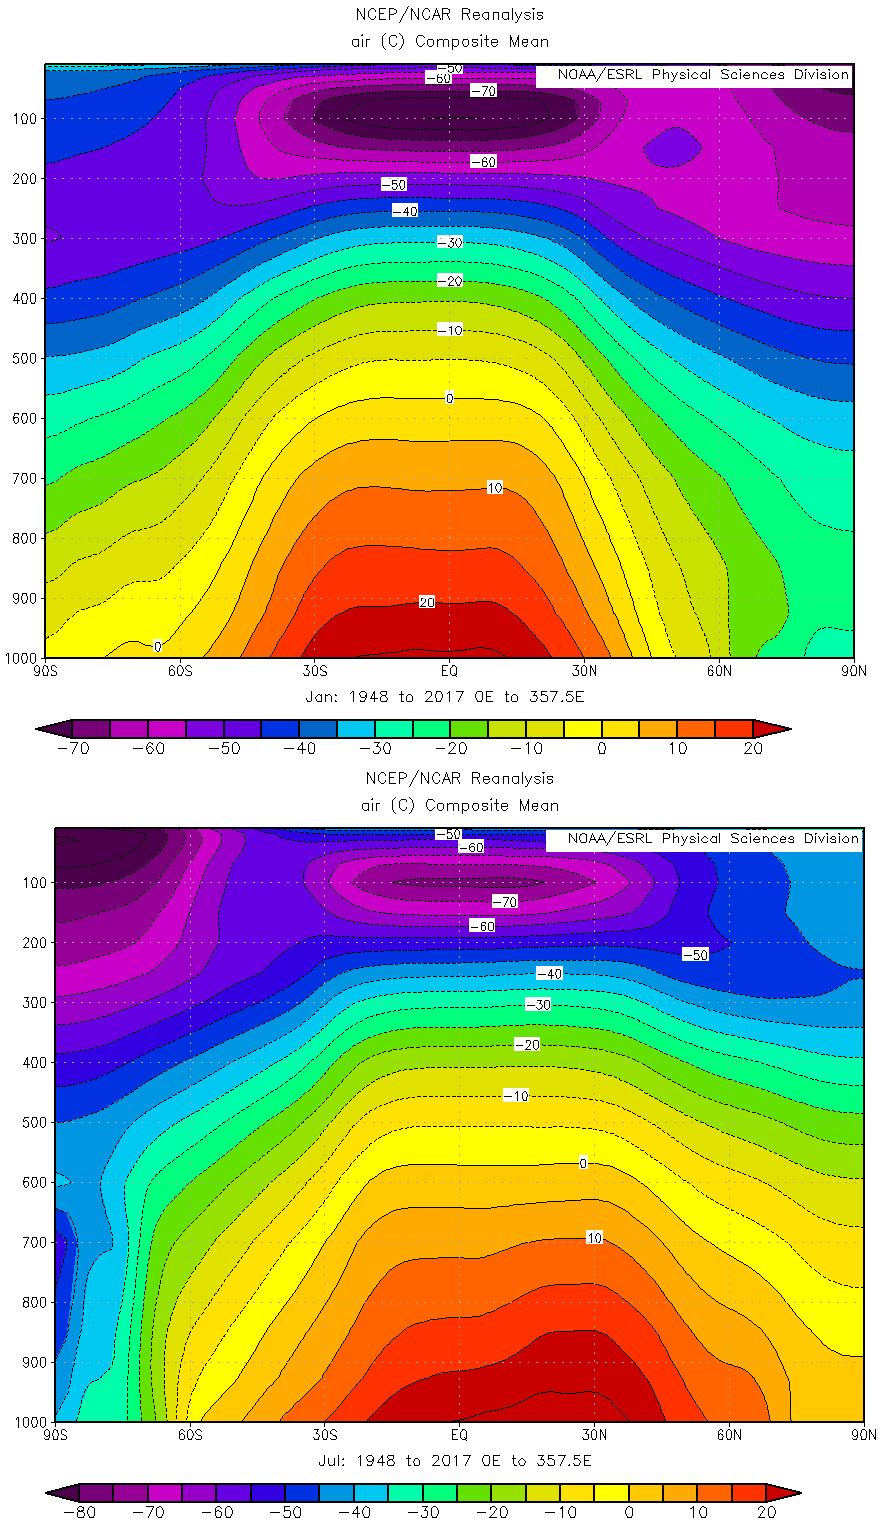
\includegraphics[width=0.8\textwidth]{airT_janjul.png}
  \caption{Zonally averaged surface air temperatures (in \SI{}{\degreeCelsius}) for the months of January and July produced using using NCEP reanalysis data averaged over the years 1948--2017.}
  \label{fig:airT}
\end{figure}

\begin{figure}[h!]
  \centering
  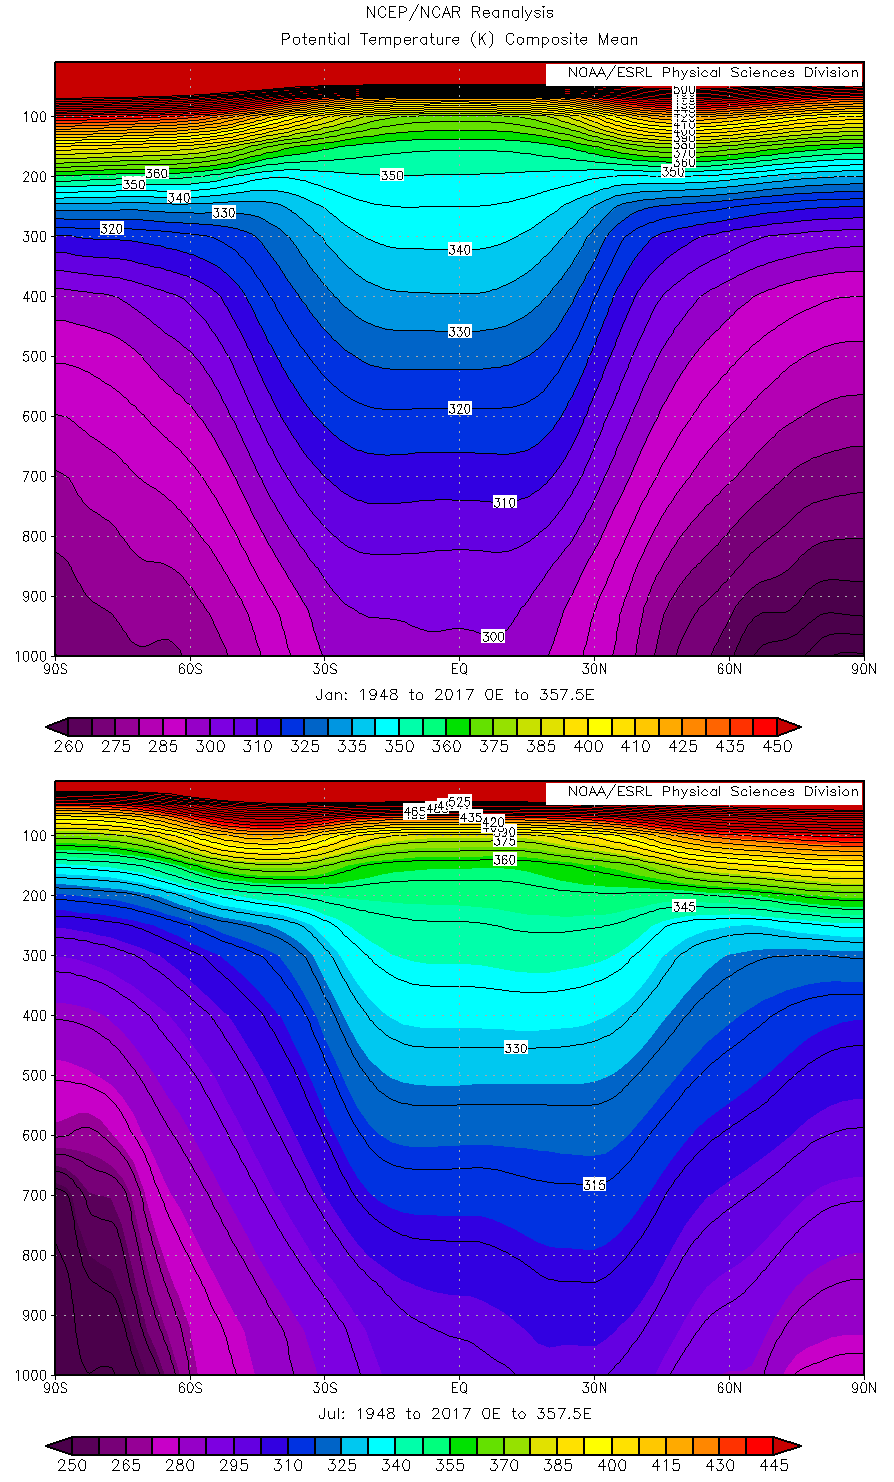
\includegraphics[width=0.8\textwidth]{theta_janjul.png}
  \caption{Zonally averaged potential temperatures (in units of Kelvin) for the months of January and July produced using using NCEP reanalysis data averaged over the years 1948--2017.}
  \label{fig:theta}
\end{figure}

\begin{figure}[h!]
  \centering
  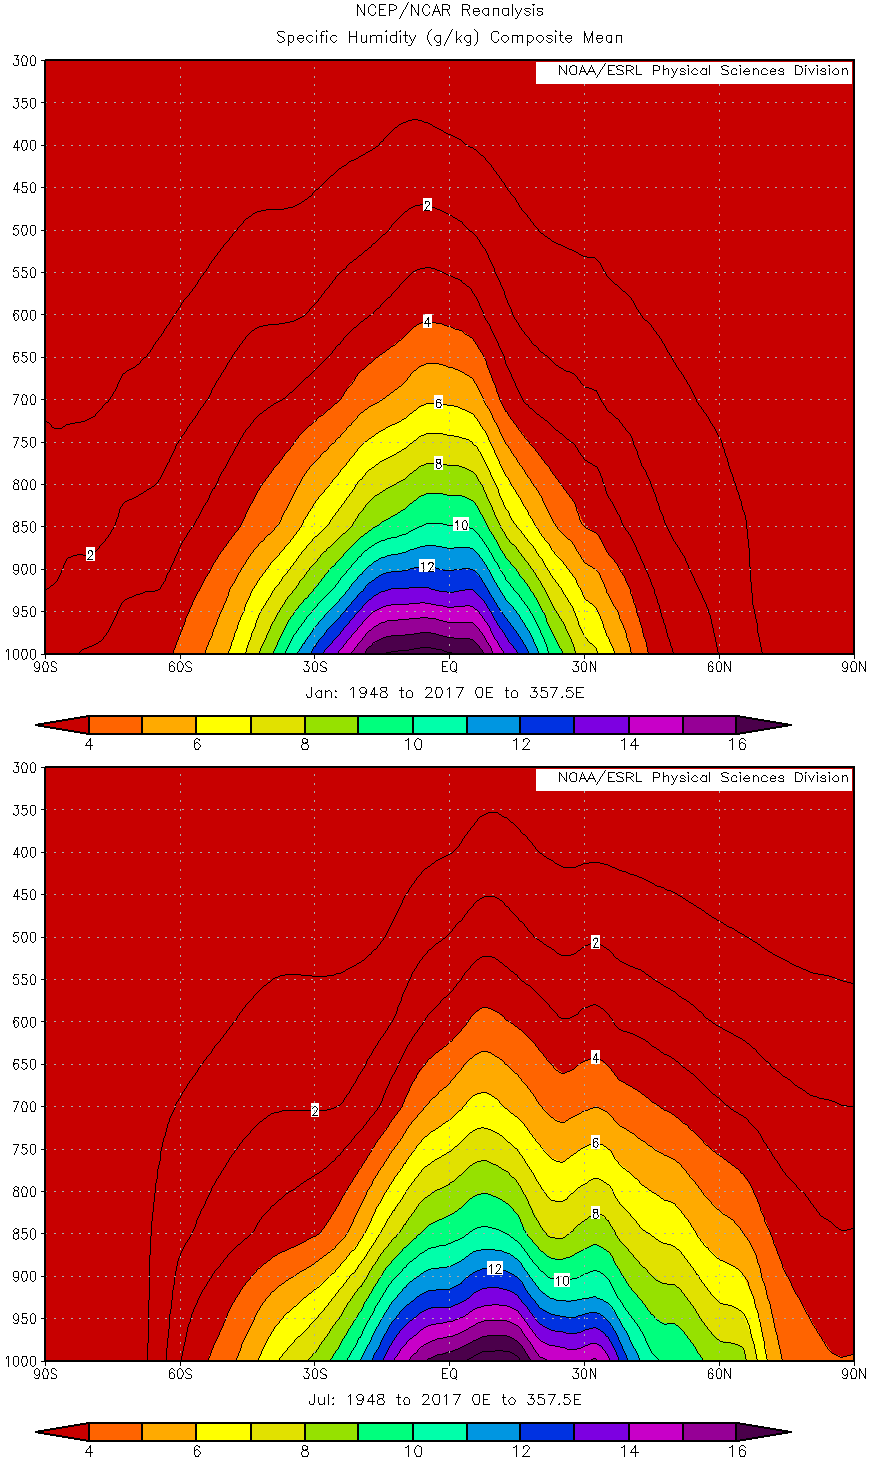
\includegraphics[width=0.8\textwidth]{qstar_janjul.png}
  \caption{Zonally averaged specific humidity (in \SI{}{\g/\kg}) for the months of January and July produced using using NCEP reanalysis data averaged over the years 1948--2017.}
  \label{fig:qstar}
\end{figure}

\begin{figure}[h!]
  \centering
  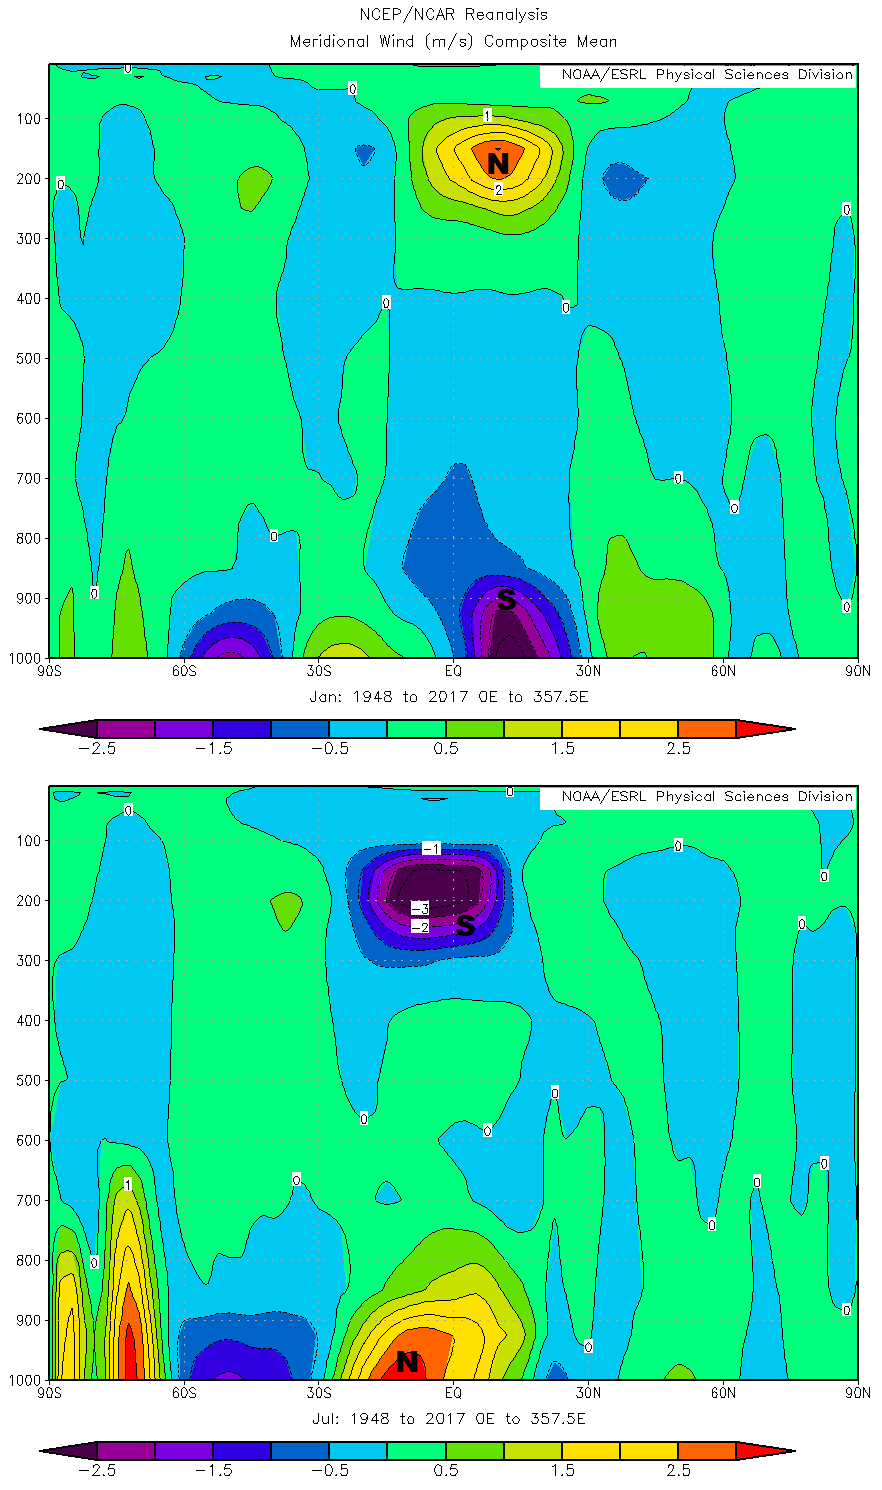
\includegraphics[width=0.8\textwidth]{mer_wind_janjul.png}
  \caption{Zonally averaged meridional wind (in \SI{}{\m/\s}) for the months of January and July produced using using NCEP reanalysis data averaged over the years 1948--2017. Regions of poleward air transport are marked \textbf{N} (northward) with regions of air transport towards the equator being marked \textbf{S} (southward).}
  \label{fig:mer_wind}
\end{figure}

\begin{figure}[h!]
  \centering
  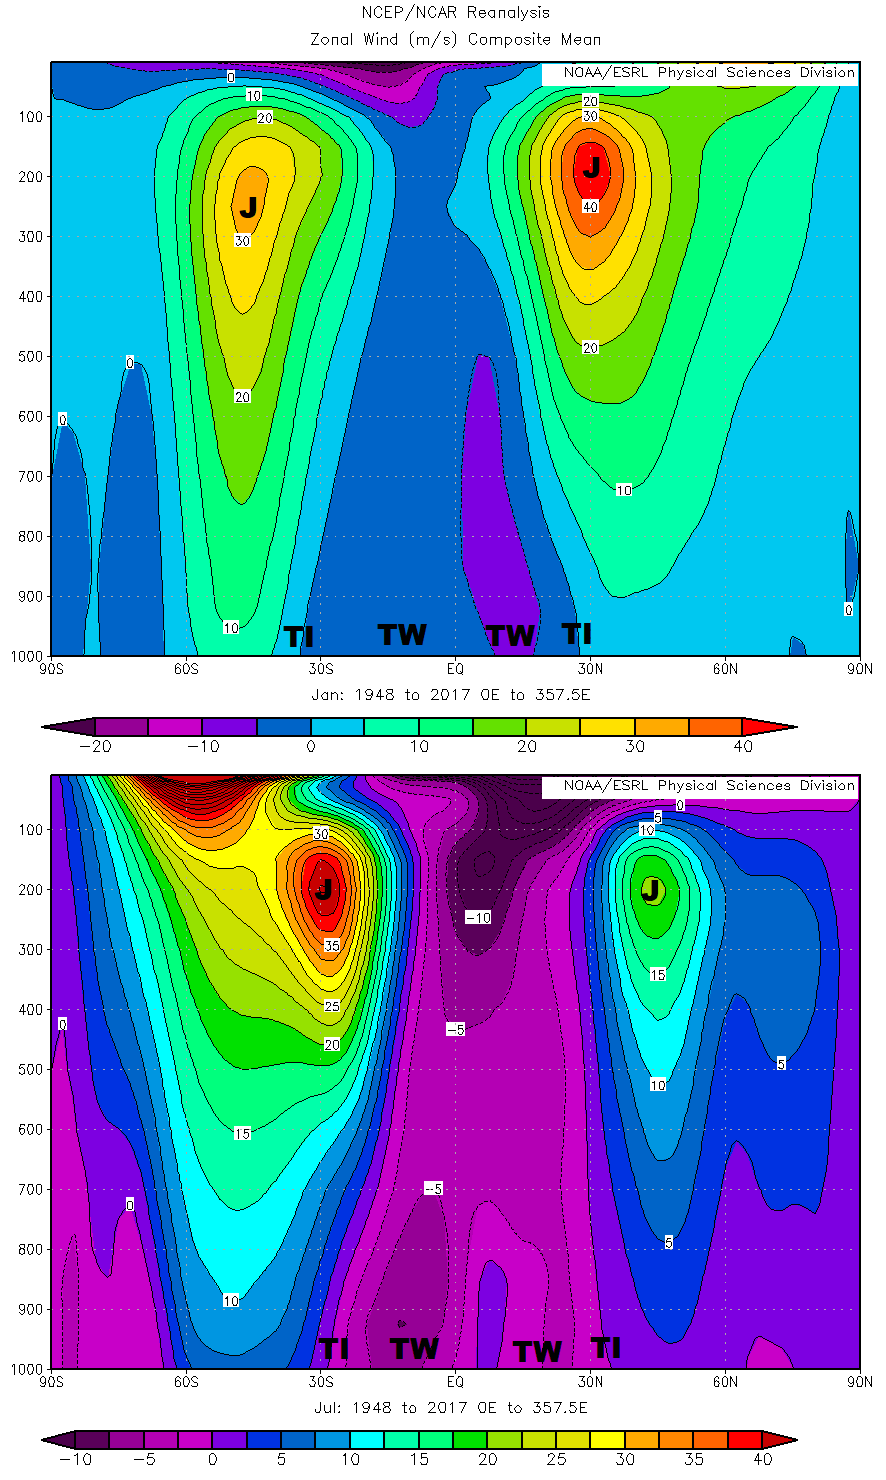
\includegraphics[width=0.8\textwidth]{zonal_wind_janjul.png}
  \caption{Zonally averaged zonal wind (in \SI{}{\m/\s}) for the months of January and July produced using using NCEP reanalysis data averaged over the years 1948--2017. The subtropical jets are marked with a \textbf{J}. Trade wind regions are marked \textbf{TW} and the trade inversions are marked \textbf{TI}.}
  \label{fig:zonal_wind}
\end{figure}

\begin{figure}[h!]
  \centering
  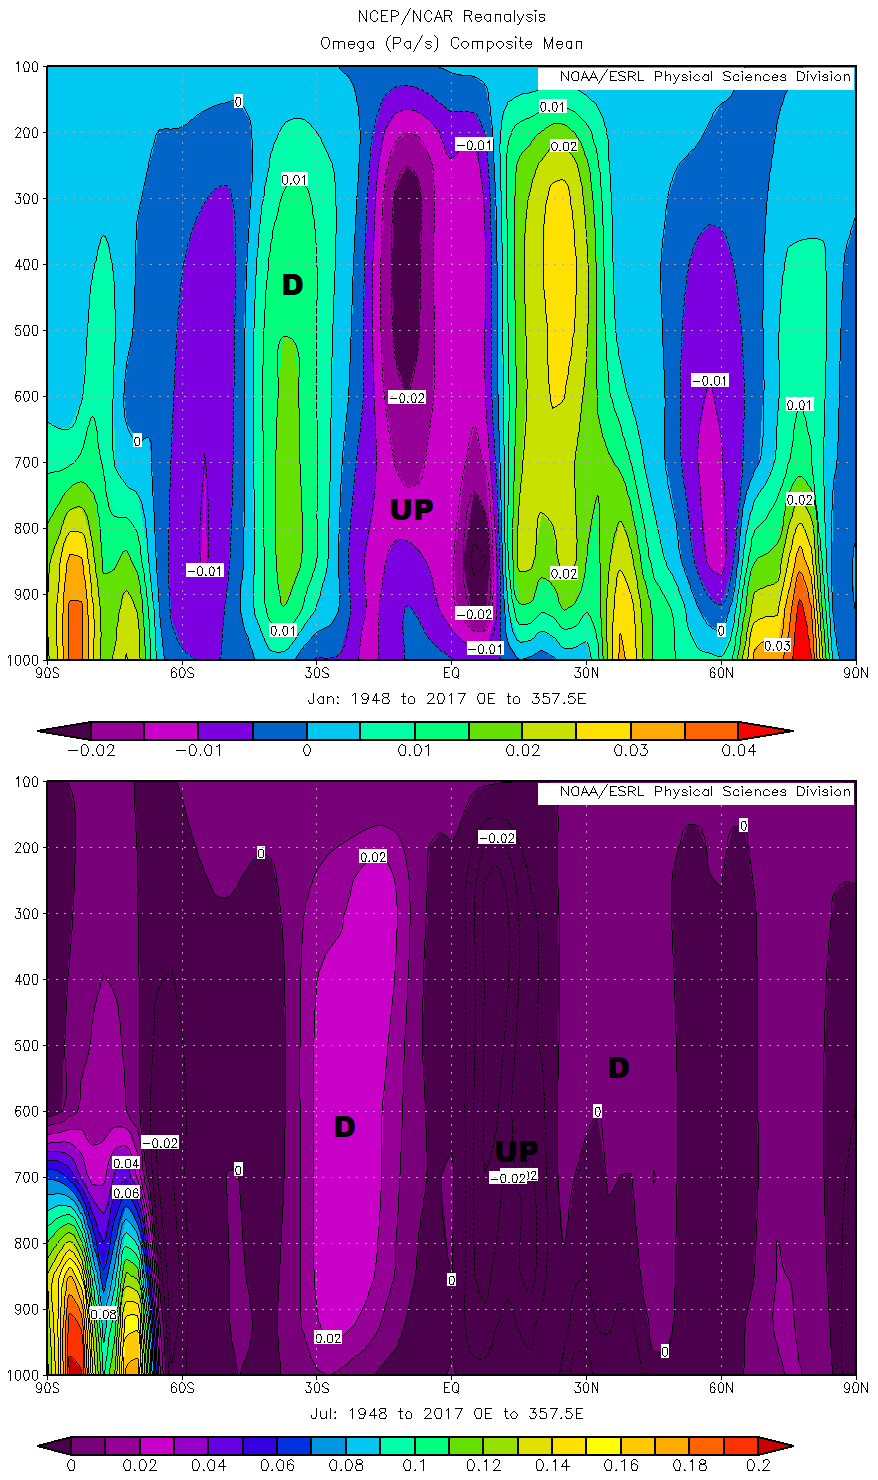
\includegraphics[width=0.8\textwidth]{omega_janjul.png}
  \caption{Zonally averaged vertical velocities (in \SI{}{\Pa/\s}) for the months of January and July produced using using NCEP reanalysis data averaged over the years 1948--2017. Regions of rising warm air are marked \textbf{UP} while regions of sinking cold air are marked \textbf{D}. Apologies for the horrible choice of contours for the July panel.}
  \label{fig:omega}
\end{figure}


\begin{thebibliography}{9}
\bibitem{Kalnay}
Kalnay, E., Kanamitsu, M., Kistler, R., Collins, W., Deaven, D., Gandin, L., Iredell, M., Saha, S., White, G., Woollen, J. and Zhu, Y., 1996. The NCEP/NCAR 40-year reanalysis project. \textit{Bulletin of the American meteorological Society}, 77(3), pp. 437--471.
\end{thebibliography}

\end{document}